
\subsection{Crocodylidae --- Crocodiles}
\begin{center}
\begin{longtabu} to \textwidth {| | p{3.5cm} | X | |}
	\hline
	Taxonomy/Ancestry & 
	\begin{itemize}[noitemsep]
		\item subfamilies -- crocodylinae, mekosuchinae (ex.), tomistominae
		\item \textbf{tomistominae} -- false gharial; genetic evidence suggests they are closer to the gharials so they may be reclassified into the Gavialidae family
		\item 3 extant genera; 16-17 species
		\item Ancient Greek = ``lizard of the Nile"
		\item separated from other crocodilians during Eocene epoch 55 million years ago
		\item closest living relatives are birds
	\end{itemize}
	
	\begin{center} 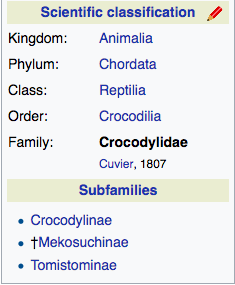
\includegraphics[scale=0.5]{crocodylia/crocodylidae/crocodylidae.png} \end{center}
	\\
	\hline
	Size & 
	5-20 ft (1.5-6.1 m)
	
	weigh up to 2000 lb (900 kg)
	
	juveniles 20 cm (7.9 in)
	\\
	\hline
	Color & \\
	\hline
	Anatomy & 
	\begin{itemize}[noitemsep]
		\item diapsid skull
		\item dorsal scales backed by osteoderms from heavy armor plating on neck and back
		\item tail strongly muscled and flattened for swimming
		\item aquatic adaptations
			\begin{itemize}[noitemsep]
			\item nostril/ear valves
			\item nictitating membrane to cover eye
			\item glottal valve in throat
			\item able to concentrate and excrete salt; salt glands on tongue filter salt to allow for survival in saltwater environments
			\end{itemize}
		\item webbing on toes of the hind feet speeds swimming + gives advantage on dry land
		\item cerebral cortex w/ 4-chambered heart
		\item slit pupils w/ tapetum lucidum
		\item teeth are replaced throughout lifespan
		\item poikilothermic + ectothermic
		\item live 70-80 yrs
		\item distinguishing from alligators
			\begin{itemize}[noitemsep]
			\item narrower + longer heads
			\item v-shaped snouts
			\item lower teeth protrude when mouth closed
			\item large 4th tooth visible
			\item salt glands = saltwater habitat
			\item sensory pits all over body
			\item jagged fringe on hind legs + feet
			\item more aggressive + dangerous
			\end{itemize}
	\end{itemize}
	\\	
	\hline
	Dimorphism & 
	males grow larger + faster
	\\
	\hline
	Behavior & 
	\begin{itemize}[noitemsep]
		\item nocturnal hunter-scavengers
		\item often bask on shoreline
		\item aestivate during drought or arid conditions
		\item adult males bellow, growl, or hiss for dominance
		\item hatchlings grunt, squawk, communicate thru ultrasound
	\end{itemize}
	\\
	\hline
	Habitat & 
	Hill streams, large rivers, marshes, ponds, lakes, canals, reservoirs, saline habitats (i.e. mangrove creeks/saltpans)
	
	Deep water = safety + drought resistance but some species live in places where water regularly dries (Crocodylus suchus) by living in deep tunnels or caves; drought can also force species to move inland 
	\\
	\hline
	Distribution & 
	tropical + subtropical regions in Africa, Asia, Americas, Australia
	\\
	\hline
	Feeding Ecology &
	\begin{itemize}[noitemsep]
		\item opportunistic apex of the food chain
		\item young are agile + can jump to eat dragonflies, termites, spiders, other insects
		\item adolescents begin to feed on crabs, fish, frogs, reptiles, birds, + mammals
		\item scavenge for carrion
		\item teeth/jaws designed for seizing, tearing, + crushing rather than chewing
		\item some species have narrow jaws + sharp teeth to hunt fish
		\item	Sensory pores in or around mouth to help detect prey
		\item	Some species herd fish to shore w/ their bodies, often communally
		\item	Control predators of commercially important fish + help maintain cleanliness as scavengers
	\end{itemize}
	 \\
	\hline
	Reproductive Biology & 
	\begin{itemize}[noitemsep]
		\item males defend territories + compete for mates
		\item fixed breeding seasons where males mate w/ multiple females
		\item females lay eggs 40-70 days after mating; incubation period depends on nest temp (avg. 60-90 days)
			\begin{itemize}[noitemsep]
			\item higher temperatures = male, lower temperatures = female
			\item \textbf{hole-diggers} -- females dig in sand, earth, or gravel embankments above the hindwater line w/ clawed hind-limbs; eggs emerge lubricated + hatch with the wet season
			\item \textbf{mound-nesters} -- females gather vegetation, soil, or compost  and digs a hole on top to lay eggs; eggs are laid at the start of the wet season and hatch when the water is highest
			\end{itemize}
		\item females, sometimes males, guard nest during incubation
		\item young call w/ quacking grunts when ready to emerge so parents release young and carry to water
		\item young are cared for in creche formation w/ parents guarding young for 90 days
		\item adults are conditioned to respond to young distress calls
		\item mortality rate = 90\% due to predators
	\end{itemize}
	\\
	\hline
	Conservation Status &
	populations are reduced due to overhunting (for skin) and habitat loss due to human industrialization. sustainable-use programs responsible for recovery and continued survival of species like Nile, saltwater, and New Guinea crocodiles. 3 CR; 2 EN; 3 VU; 1 CD; 1 DD. 
	
	In Ancient Egypt (Sobek and Taweret), Hinduism (Varuna, Ganga, Yamuna, Goa), Aztec (Cipactli)
	 \\
	\hline 
\end{longtabu}
\end{center}